% !TEX root = ../../report.tex
\begin{Spacing}{\mylinespace}
\section{CPU vs. GPU}
CPUs und GPUs weisen grundlegend verschiedene Architekturen auf.
\begin{figure}[h!]
	\vspace*{30px}
	\centering
	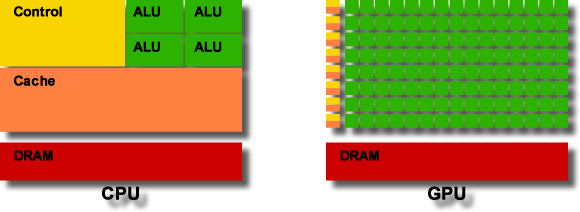
\includegraphics[width=320px]{graphics/GPUvsCPU.png}	
	\caption{CPU- vs. GPU-Architektur}
	\label{fig:GPUvsCPU}
\end{figure}

Während eine CPU einen relativ großen Befehlssatz hat um Ganz- oder Fließkommazahlen zu verarbeiten, eine GPU  besitzt hingegen einen sehr kleinen Befehlssatz und kann lediglich Fließkommazahlen verarbeiten.
Der große Vorteil einer GPU jedoch ist, dass sie die Möglichkeit besitzt, Berechnungsaufgaben an verschiedene kleinere CO-Prozessoren, sogenannte Shader-Units abzugeben. Durch das zuweisen einer Aufgabe pro Shader-Unit erlaubt eine GPU somit das hoch-parallele abarbeiten von Aufgaben - solange diese unabhängig voneinander sind.
Diese parallele Programmierung hat jedoch auch Nachteile.
Nicht nur das es einer speziellen Programmierung benötigt - sogenannte Shader-Programmierung (Shader-Programme).
Sondern es setzt auch Vorraus, das jede Shader-Unit das gleiche Shader-Programm ausführt. Besitzen jedoch die zu verarbeitenden Berechnungen genug Unabhänigkeit, so kann eine erhebliche Beschleunigung durch den Einsatz einer GPU, welche meist hunderte von Shader-Units besitzt, erzielt werden.


\section{GPU-Programmierung}

Die GPU-Programmierung unterscheidet sich in vielen Punkten von der CPU-Programmierung. Für ein besseres Verständnis ist es von Vorteil, wenn man die einzelnen Arbeitsschritte einer GPU von der Eingabe bis zur Ausgabe kennt. Diese wollen wir folgend, mit Hilfe eines kleinen Beispiels erläutern.

\begin{figure}[h!]
	\vspace*{20px}
	\centering
	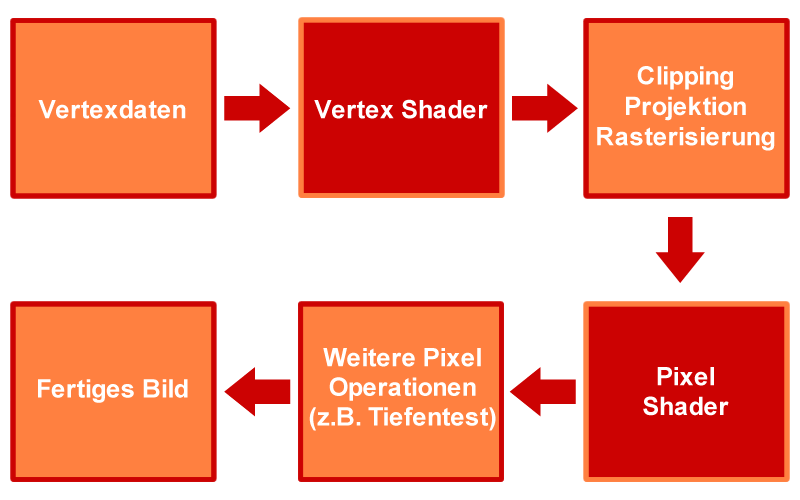
\includegraphics[width=330px]{graphics/pipeline.png}	
	\caption{Die GPU Pipeline}
	\label{fig:pipeline}
\end{figure}

Abbildung \ref{fig:pipeline} zeigt die einzelnen Arbeitsschritte einer GPU. Starten wir, mit unserem Beispiel im ersten Schritt \textit{Vertexdaten}. Um das Beispiel möglichst simple zu gestalten, wollen wir ein einfaches rotes Rechteck generieren und ausgeben. Dazu muss man wissen, das eine GPU immer nur einzelne Punkte oder Dreiecke zeichnen kann. Um unser Rechteck zu erzeugen benötigen wir also zwei Dreiecke, die jeweils aus drei Punkten bestehen. (s. Abbildung \ref{fig:Viereck}).

\begin{figure}[h!]
	\vspace*{30px}
	\centering
	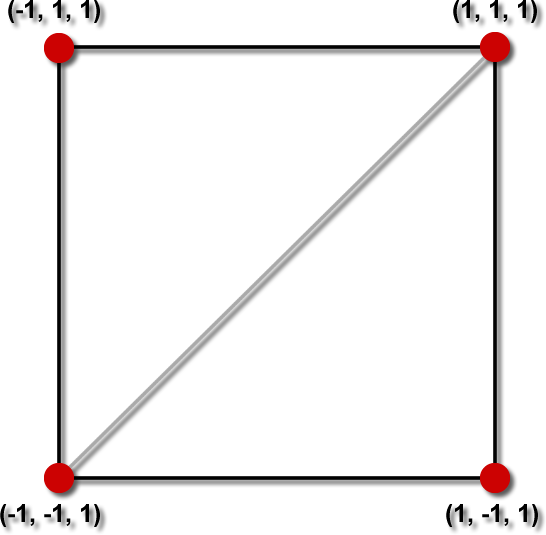
\includegraphics[height=130px]{graphics/Quad2.png}	
	\caption{Aufbau des Rechtecks}
	\label{fig:Viereck}
\end{figure}

\subsection{VertexBuffer}
Um die insgesamt sechs Punkte unseres Rechtecks an die GPU zu übergeben, erzeugen wir einen sogenannten \textit{Vertex Buffer}. Dieser stellt einen Speicherbereich für unsere einzelnen Punkte auf der GPU dar. Die Punkte werden in dem \textit{Vertex Buffer} so abgelegt, dass sie sequentiell abgearbeitet, unsere beiden Dreiecke ergeben. Hierbei muss auch die Reihenfolge der Punkte pro Dreieck beachtet werden. Je nach Einstellung, kann diese im Uhrzeigersinn oder gegen den Uhrzeigersinn angegeben werden. Abbildung \ref{fig:VertexBuffer} zeigt den benötigten \textit{Vertex Buffer} zur Erzeugung der beiden Dreiecke im Uhrzeigersinn.

\begin{figure}[h!]
	\vspace*{15px}
	\centering
	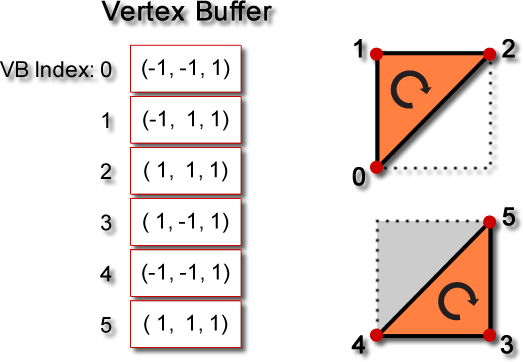
\includegraphics[height=120px]{graphics/vertexbuffer2.png}	
	\caption{Der VertexBuffer unseres Rechtecks}
	\label{fig:VertexBuffer}
\end{figure}

\subsection{IndexBuffer}
Wie man in Abbildung \ref{fig:VertexBuffer} erkennen kann, enthält unser erzeugter \textit{Vertex Buffer} duplizierte Einträge an den Stellen (0-4) und (2-5). Bei dem, in unserem Beispiel verwendeten Rechteck, fällt dieser unnötige Speicherverbrauch nicht großartig ins Gewicht. Bei weitaus komplexeren Modellen, können diese doppelten Einträge jedoch schnell zu einem Problem werden. Um doppelte Einträge im \textit{Vertex Buffer} zu verhindern, werden sogenannte \textit{Index Buffer} eingesetzt. Diese enthalten Indizes die auf die einzelnen Einträge im \textit{Vertex Buffer} referenzieren. Abbildung \ref{fig:IndexBuffer} zeigt, den für unser Beispiel benötigen, Index- und Vertex Buffer. Wie man sieht sind die doppelten Einträge aus unserem \textit{Vertex Buffer} verschwunden und die Reihenfolge zum Zeichen der beiden Dreiecke, wird nun durch den \textit{Index Buffer} vorgegeben. 
 

\begin{figure}[h!]
	\vspace*{15px}
	\centering
	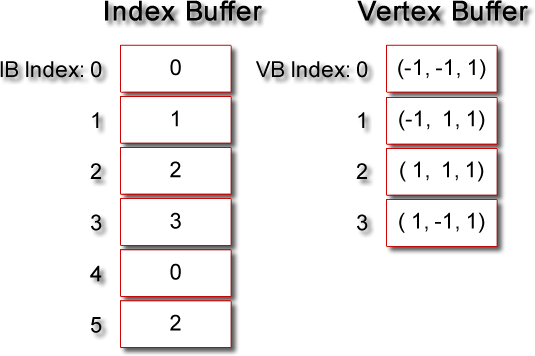
\includegraphics[height=120px]{graphics/indexbuffer2.png}	
	\caption{Der Vertex- und Index Buffer unseres Rechtecks}
	\label{fig:IndexBuffer}
\end{figure}

\subsection{Vertex Shader}
Nachdem wir unsere Daten nun erfolgreich auf die GPU übertragen haben, geht es weiter mit dem nächsten Schritt, dem \textit{Vertex Shader}. Shader sind die programmierbaren Einheiten einer GPU, in denen wir selbst Einfluss auf die Grafikpipeline nehmen können. Dazu zählen, der \textit{Vertex Shader}, auf den wir hier einen Blick werfen werden, der \textit{Pixel Shader}, den wir uns danach betrachten und bei neueren GPU's der \textit{Geometry Shader}, den wir hier nicht behandeln wollen.
\\\\
Der \textit{Vertex Shader} arbeitet auf der \textit{Vertex}-Ebene, das sind unsere einzelnen Punkte. Diese können hier noch einmal manipuliert oder transformiert werden.
Der Quellcode \ref{vertexshader} zeigt einen minimalen \textit{Vertex Shader}. Dieser bekommt unsere Punkte übergeben, transformiert diese mit der Matrix \textit{worldViewProj} vom \textit{Objectspace} in den \textit{Screenspace} und gibt die transformierten Punkte an den nächsten Schritt der Pipeline weiter.

\begin{lstlisting}[captionpos=b, caption=Vertex Shader unseres Rechtecks., label=vertexshader]
01 float4x4 worldViewProj;
02
03 float4 vertexshader(float4 position)
04 {
05   return mul(position, worldViewProj);		
06 }
\end{lstlisting}

\subsection{Clipping, Projektion, Rasterisierung}
In diesem Schritt werden unsere, in den \textit{Screenspace} transformierten Punkte, auf einzelne Bildschirmpixel abgebildet (Rasterisierung) und alle überflüssigen Pixel, die außerhalb des Bildschirmbereichs liegen, verworfen (Clipping).

\subsection{Pixel Shader}
Nachdem unsere dreidimensionalen Punkte, im vorherigen Schritt zu zweidimensionalen Bildschirmpixel gerastert wurden, kommen wir nun zur nächsten programmierbaren Einheit einer GPU, dem \textit{Pixel Shader}. Dieser arbeitet auf textit{Pixel}-Ebene und ist für deren Einfärbung zuständig. Der Quellcode \ref{pixelshader} zeigt einen minimalen \textit{Pixel Shader}. Dieser färbt alle Pixel unseres Rechtecks rot ein.

\begin{lstlisting}[captionpos=b, caption=Fragment Shader unseres Rechtecks., label=pixelshader]
01 float4 pixelshader()
02 {
03   return float4(0.8, 0.0, 0.0, 1.0);
04 }
\end{lstlisting}

\subsection{Weitere Pixel Operationen}
Auf die weiteren Pixel Operationen wie den Tiefentest, der für die Tiefensortierung der einzelnen Pixel zuständig ist, wollen wir der Einfachheit unseres Beispiels hier nicht näher eingehen.

\subsection{Fertiges Bild}
Als Resultat unseres kleinen Beispiels, erhalten wir am Ende, das in Abbildung \ref{fig:exampleRes} gezeigte, rot gefärbte Rechteck.

\begin{figure}[h!]
	\vspace*{15px}
	\centering
	
\includegraphics[height=120px]{graphics/exampleRes.png}	
	\caption{Der Ergebnis unseres kleinen Beispiels.}
	\label{fig:exampleRes}
\end{figure}

\end{Spacing}
\clearpage
%% End Of Doc